\documentclass[fleqn]{article}
\oddsidemargin 0.0in
\textwidth 6.0in
\thispagestyle{empty}
\usepackage{import}
\usepackage{amsmath}
\usepackage{graphicx}
\usepackage{flexisym}
\usepackage{calligra}
\usepackage{amssymb}
\usepackage{bigints} 
\usepackage[english]{babel}
\usepackage[utf8x]{inputenc}
\usepackage{float}
\usepackage[colorinlistoftodos]{todonotes}


\DeclareMathAlphabet{\mathcalligra}{T1}{calligra}{m}{n}
\DeclareFontShape{T1}{calligra}{m}{n}{<->s*[2.2]callig15}{}
\newcommand{\scriptr}{\mathcalligra{r}\,}
\newcommand{\boldscriptr}{\pmb{\mathcalligra{r}}\,}

\definecolor{hwColor}{HTML}{1a0252}

\begin{document}

  \begin{titlepage}

    \newcommand{\HRule}{\rule{\linewidth}{0.5mm}}

    \center


    \textsc{\LARGE Arizona State University}\\[1.5cm]

    \textsc{\LARGE Quantum Physics II}\\[1.5cm]


    \begin{figure}
      
\includegraphics[width=\linewidth]{asu.png}
    \end{figure}


    \HRule \\[0.4cm]
    { \huge \bfseries Problem Set 2}\\[0.4cm] 
    \HRule \\[1.5cm]

    \textbf{Behnam Amiri}

    \bigbreak

    \textbf{Prof: Onur Erten}

    \bigbreak


    \textbf{{\large \today}\\[2cm]}

    \vfill

  \end{titlepage}

  \begin{enumerate}
    \item \textbf{4-16} A rod of proper length $l_0$ is at rest in a frame $S^'$. It lies in the $(x^',y^')$ plane and makes
    an angle of $sin^{-1}(\dfrac{3}{5})$ with the $x^'$ axis. If $S^'$ moves with constant velocity $v$ parallel to the 
    $x$ axis of another frame $S:$
    \begin{enumerate}
      \item What must be the value of $v$ if, as measured in $S$, the rod is at $45^\circ$ to the $x$ axis?

        \textcolor{hwColor}{
          $
            \theta=sin^{-1}(\dfrac{3}{5})
            \\
            \\
            \begin{cases}
              l_x=l_0 cos(45^{\circ}) 
              \\
              \\
              l^'_x=l_0 cos(\theta)
            \end{cases}
            \\
            \\
            \\
            l_x=l^'_x \sqrt{1-\left(\dfrac{v}{c}\right)^2}
            \\
            \\
            \\
            \left(\dfrac{l_x}{l^'_x}\right)^2=1-\left(\dfrac{v}{c}\right)^2
            \\
            \\
            \\
            \left(\dfrac{v}{c}\right)^2=1-\left(\dfrac{l_x}{l^'_x}\right)^2
            \\
            \\
            \\
            v^2=c^2\left[1-\left(\dfrac{l_x}{l^'_x}\right)^2\right]
            =c^2\left[1-\left(\dfrac{l_0 cos(45^{\circ})}{l_0 cos(\theta)}\right)^2\right]
            =c^2\left[1-\left(\dfrac{cos(45^{\circ})}{cos(\theta)}\right)^2\right]
            \\
            \\
            \\
            \therefore ~~~ v \approx 1.40 \times 10^{8} ~~~ \checkmark
          $
        }


      \item What is the length of the rod as measured in $S$ under these conditions?


        \textcolor{hwColor}{
          $
            l=\dfrac{l_0}{\sqrt{1-\left(\dfrac{v}{c}\right)^2}}
            \\
            \\
            \\
            \therefore ~~~~ l=1.14 l_0 ~~~ \checkmark
          $
        }

    \end{enumerate}

    \pagebreak

    \item \textbf{5-7} An inertial system $S_1$ has a constant velocity $v_1$ along the $x$ axis relative to an inertial system $S$.
    Inertial system $S_2$ has a velocity $v_2$ relative to $S_1$. Two successive Lorentz-Einstein transformations enable us to
    go from $(x, y, z, t)$ to $(x_1, y_1, z_1, t_1)$ and then from $(x_1, y_1, z_1, t_1)$ to $(x_2, y_2, z_2, t_2)$. Show that 
    this gives the same result as a single Lorentz-Einstein transformation from $(x, y, z, t)$ to $(x_2, y_2, z_2, t_2)$,
    provided we take the velocity $v$ of $S_2$ relative to $S$ as
    $$v=\dfrac{v_1+v_2}{1+\dfrac{v_1 v_2}{c^2}}$$

      \textcolor{hwColor}{
        We are asked to show that two successive Lorentz-Einstein transformations gives the same result as a single Lorentz-Einstein transformation.
        Let's write down the Lorentz transformations:
        \\
        \\
        \\
        $
          \begin{cases}
            x_0^'=\gamma_1 \left(x_0-\beta_1 x_1\right)
            \\
            \\
            x_1^'=\gamma_1 \left(x_1-\beta_1 x_0\right)
          \end{cases} ~~~~~ x_0=ct, ~~~ \beta_1=\dfrac{v_1}{c}, ~~~ \gamma_1=\dfrac{1}{\sqrt{1-\left(\dfrac{v_1}{c}\right)^2}}
        $
        \\
        \\
        Defining another frame as the double-prime, then the Lorentz transformation:
        \\
        \\
        $
          \begin{cases}
            x_0^{''}=\gamma_2 \left(x_0^'-\beta_2 x_1^'\right)
            \\
            \\
            x_1^{''}=\gamma_2 \left(x_1^'-\beta_2 x_0^'\right)
          \end{cases} ~~~~~ x_0=ct, ~~~ \beta_2=\dfrac{v_2}{c}, ~~~ \gamma_2=\dfrac{1}{\sqrt{1-\left(\dfrac{v_2}{c}\right)^2}}
          \\
          \\
          \\
          \begin{cases}
            x_0^{''}=\gamma_1 \gamma_2 \left[\left(1+\beta_1 \beta_2\right)x_0-\left(\beta_1 \beta_2\right)x_1\right]
            \\
            \\
            \\
            x_1^{''}=\gamma_1 \gamma_2 \left[\left(1+\beta_1 \beta_2\right)x_1-\left(\beta_1 \beta_2\right)x_0\right]
          \end{cases}
        $
        \\
        \\
        \\
        Let's have the double-primed frame traveling at a speed $v$ relative to the unprimed frame, 
        then the Lorentz transformation relating the two is:
        \\
        \\
        \\
        $
          \begin{cases}
            x_0^{''}=\gamma \left(x_0-\beta x_1\right)
            \\
            \\
            x_1^{''}=\gamma \left(x_1-\beta x_0\right)
          \end{cases} ~~~~~ x_0=ct, ~~~ \beta=\dfrac{v}{c}, ~~~ \gamma=\dfrac{1}{\sqrt{1-\left(\dfrac{v}{c}\right)^2}}
        $
        \\
        \\
        \\
        Comparing this to the double transformation, we have the following result:
        \\
        \\
        \\
        $
          \begin{cases}
            \gamma=\gamma_1 \gamma_2 \left(1+\beta_1 \beta_2\right)
            \\
            \\
            \gamma \beta=\gamma_1 \gamma_2 \left(\beta_1+\beta_2\right)
            \\
            \\
            \gamma=\gamma_1 \gamma_2 \left(1+\beta_1 \beta_2\right)
            \\
            \\
            \gamma \beta=\gamma_1 \gamma_2 \left(\beta_1+\beta_2\right)
          \end{cases}
        $
        \\
        \\
        \\
        Hence,
        \\
        \\
        $
          \dfrac{1}{\sqrt{1-\left(\dfrac{v}{c}\right)^2}}
          =\dfrac{1}{\sqrt{1-\left(\dfrac{v_1}{c}\right)^2}} \dfrac{1}{\sqrt{1-\left(\dfrac{v_2}{c}\right)^2}} \left(1+\dfrac{v_1 v_2}{c^2}\right)
          \\
          \\
          \\
          1-\left(\dfrac{v}{c}\right)^2=\dfrac{ \left(1-\left(\dfrac{v_1}{c}\right)^2\right) \left(1-\left(\dfrac{v_2}{c}\right)^2\right)  }{\left(1+\dfrac{v_1 v_2}{c^2}\right)^2}
          \\
          \\
          \\
          v=\sqrt{c^2-c^2\dfrac{
            \left[1-\left(\dfrac{v_1}{c}\right)^2\right]
            \left[1-\left(\dfrac{v_2}{c}\right)^2\right]
          }{
            \left[1+\dfrac{v_1 v_2}{c^2}\right]^2
          }}
          \\
          \\
          \\
          \\
          =\sqrt{
            c^2-\dfrac{c^2+\left(\dfrac{v_1 v_2}{c}\right)^2-v_1^2-v_2^2
          }{
            1+2\dfrac{v_1 v_2}{c^2+\left(\dfrac{v_1 v_2}{c^2}\right)^2}
          }}
          \\
          \\
          \\
          \\
          \therefore ~~~~ v=\dfrac{v_1+v_2}{1+\dfrac{v_1 v_2}{c^2}} ~~~ \checkmark
        $
      }

    \pagebreak

    \item \textbf{5-9} Three identical radio transmitters $A, B,$ and $C,$ each transmitting at the frequency $v_0$ in its own
    rest frame, are in motion as shown.

    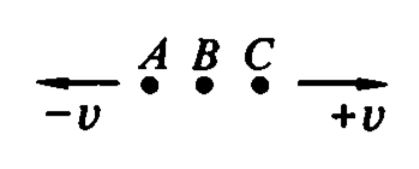
\includegraphics[height=3cm, width=4cm]{1.JPG}

    \begin{enumerate}
      \item What is the frequency of $B^'$s signals as received by $C$?
      
        \textcolor{hwColor}{
          $
            \\
            v=v_0 \sqrt{\dfrac{1-\left(\dfrac{v}{c}\right)}{1+\left(\dfrac{v}{c}\right)}}
            \\
          $
        }


      \item What is the frequency of $A^'$s signals as received by $C$?

        \textcolor{hwColor}{
          $
            \\
            v=v_0 \sqrt{\dfrac{1-\left(\dfrac{v}{c}\right)}{1+\left(\dfrac{v}{c}\right)}} \sqrt{\dfrac{1-\left(\dfrac{v}{c}\right)}{1+\left(\dfrac{v}{c}\right)}}
            \\
            \\
            \\
            \therefore ~~~~ v=v_0 \dfrac{1-\left(\dfrac{v}{c}\right)}{1+\left(\dfrac{v}{c}\right)} ~~~ \checkmark
            \\
          $
        }

    \end{enumerate}


  \end{enumerate}

\end{document}